\scanpage{96}
% archive sheet number: 98

% printed form
{\scriptsize
\begin{verbatim}
//*   FATAR   0338        I
           00000000      00000000      00000000     2222222222
         0000000000    0000000000    0000000000   222222222222
       00      0000  00      0000  00      0000  22        22
      00     00 00  00     00 00  00     00 00           22
     00    00  00  00    00  00  00    00  00           22
    00   00   00  00   00   00  00   00   00          22
   00  00    00  00  00    00  00  00    00        22
  00 00     00  00 00     00  00 00     00      22
 0000      00  0000      00  0000      00    22
000       00  000       00  000       00   22
0000000000    0000000000    0000000000   222222222222
00000000      00000000      00000000    222222222222
\end{verbatim}
}

{\scriptsize
\begin{verbatim}
FFFFFFFFFFFF   AAAAAAAAAA   TTTTTTTTTTTT   AAAAAAAAAA   RRRRRRRRRRR
FFFFFFFFFFFF  AAAAAAAAAAAA  TTTTTTTTTTTT  AAAAAAAAAAAA  RRRRRRRRRRRR
FF            AA        AA       TT       AA        AA  RR        RR
FF            AA        AA       TT       AA        AA  RR        RR
FF            AA        AA       TT       AA        AA  RR        RR
FFFFFFFF      AAAAAAAAAAAA       TT       AAAAAAAAAAAA  RRRRRRRRRRRR
FFFFFFFF      AAAAAAAAAAAA       TT       AAAAAAAAAAAA  RRRRRRRRRRR
FF            AA        AA       TT       AA        AA  RR    RR
FF            AA        AA       TT       AA        AA  RR     RR
FF            AA        AA       TT       AA        AA  RR      RR
FF            AA        AA       TT       AA        AA  RR       RR
FF            AA        AA       TT       AA        AA  RR        RR
\end{verbatim}
}

% crop-candidate: scan 96
\figure{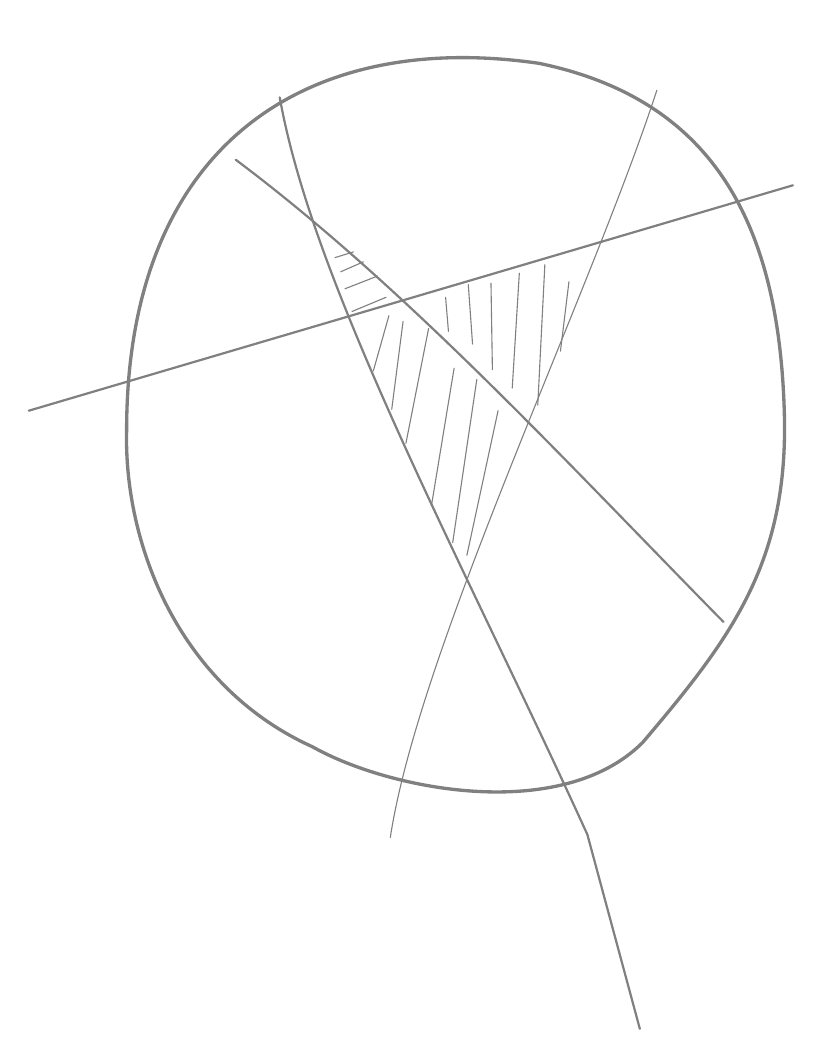
\begin{tikzpicture}[x=0.018cm,y=-0.018cm,line cap=round,line join=round]
\draw[gray,line width=1.2pt] (784,320) .. controls (784,119) and (910,37) .. (1075,61) .. controls (1200,87) and (1245,177) .. (1248,311) .. controls (1250,414) and (1210,467) .. (1148,540) .. controls (1091,597) and (970,574) .. (915,543) .. controls (820,500) and (782,399) .. (784,320) -- cycle;
\draw[gray,thick] (861,129) .. controls (981,219) and (1092,340) .. (1205,455);
\draw[gray,thick] (892,85) .. controls (916,220) and (1024,418) .. (1109,605) -- (1146,742);
\draw[gray] (1158,80) .. controls (1111,224) and (990,475) .. (970,607);
\draw[gray,thick] (715,306) -- (1254,147);
\draw[gray] (931,198)--(944,194) (935,208)--(951,201) (938,220)--(961,211) (943,236)--(967,226) (969,239)--(958,278) (979,243)--(971,305) (997,248)--(981,329) (1015,276)--(999,373) (1031,284)--(1014,399) (1046,306)--(1024,408) (1009,226)--(1011,250) (1025,217)--(1028,259) (1041,216)--(1042,277) (1061,209)--(1056,290) (1079,203)--(1074,302) (1096,215)--(1090,264);
\end{tikzpicture}}

% crop-candidate: scan 96
\figure{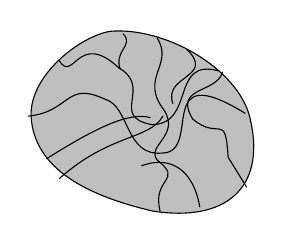
\begin{tikzpicture}[x=0.018cm,y=-0.018cm,line cap=round,line join=round]
\draw[fill=gray!50] (123,374) .. controls (122,343) and (162,315) .. (181,314) .. controls (221,312) and (272,343) .. (278,378) .. controls (288,424) and (261,449) .. (209,441) .. controls (162,430) and (125,411) .. (123,374) -- cycle;
\draw (121,374) .. controls (151,371) and (147,349) .. (175,362) .. controls (193,367) and (189,403) .. (216,400) .. controls (244,399) and (209,332) .. (274,372);
\draw (143,335) .. controls (153,351) and (156,313) .. (185,340) .. controls (209,354) and (178,374) .. (208,380) .. controls (239,380) and (221,333) .. (255,342);
\draw (188,316) .. controls (196,324) and (181,328) .. (186,341) (212,319) .. controls (224,338) and (199,347) .. (217,370) .. controls (228,388) and (204,395) .. (212,405) .. controls (231,420) and (208,417) .. (214,441);
\draw (233,327) .. controls (253,347) and (216,345) .. (223,365) (258,343) .. controls (254,358) and (223,353) .. (237,376) .. controls (256,392) and (260,370) .. (262,403) -- (275,424);
\draw (134,404) .. controls (169,382) and (192,371) .. (207,375) (143,418) .. controls (179,386) and (206,391) .. (216,374) (201,409) .. controls (220,402) and (237,410) .. (242,438);
\end{tikzpicture}}

% crop-candidate: scan 96
\figure{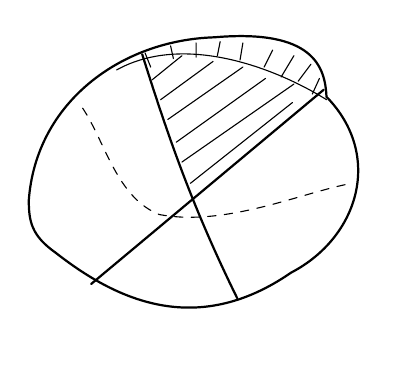
\begin{tikzpicture}[x=0.018cm,y=-0.018cm,line cap=round,line join=round]
\draw[thick] (419,353) .. controls (424,284) and (484,240) .. (550,238) .. controls (620,232) and (628,259) .. (629,280) .. controls (669,321) and (652,379) .. (604,404) .. controls (536,451) and (479,422) .. (438,390) .. controls (421,378) and (419,368) .. (419,353) -- cycle;
\draw[thick] (499,250) .. controls (517,307) and (534,357) .. (566,422) (463,412)--(627,275);
\draw (481,261) .. controls (528,235) and (592,259) .. (629,282);
\draw[dashed] (457,288) .. controls (473,312) and (481,351) .. (511,363) .. controls (558,372) and (613,347) .. (647,341);
\draw (501,249)--(505,259) (519,244)--(521,253) (537,242)--(537,252) (554,241)--(552,251) (570,242)--(568,254) (591,247)--(585,259) (606,251)--(597,266) (618,257)--(609,269) (624,267)--(619,278);
\draw (506,268)--(527,251) (512,282)--(549,255) (517,296)--(570,259) (523,312)--(586,267) (527,326)--(606,271) (533,341)--(605,284);
\end{tikzpicture}}

% crop-candidate: scan 96
\figure{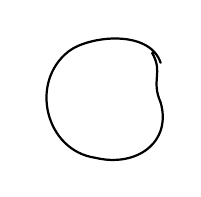
\begin{tikzpicture}[x=0.018cm,y=-0.018cm,line cap=round,line join=round]
\draw[thick] (690,433) .. controls (682,409) and (639,414) .. (625,425) .. controls (597,447) and (609,495) .. (644,500) .. controls (673,507) and (698,489) .. (690,461) .. controls (683,445) and (692,440) .. (684,426);
\end{tikzpicture}}

{\tiny
\begin{verbatim}
****A   END   JOB  338  FATAR                          ROOM        3.01.58 PM 19 AUG 82  R6.PR1    SYS JES2  JOB  338   END   A****
****A   END   JOB  338  FATAR                          ROOM        3.01.58 PM 19 AUG 82  R6.PR1    SYS JES2  JOB  338   END   A****
****A   END   JOB  338  FATAR                          ROOM        3.01.58 PM 19 AUG 82  R6.PR1    SYS JES2  JOB  338   END   A****
****A   END   JOB  338  FATAR                          ROOM        3.01.58 PM 19 AUG 82  R6.PR1    SYS JES2  JOB  338   END   A****
****A   END   JOB  338  FATAR                          ROOM        3.01.58 PM 19 AUG 82  R6.PR1    SYS JES2  JOB  338   END   A****
****A   END   JOB  338  FATAR                          ROOM        3.01.58 PM 19 AUG 82  R6.PR1    SYS JES2  JOB  338   END   A****
\end{verbatim}
}

% crop-candidate: scan 96
\figure{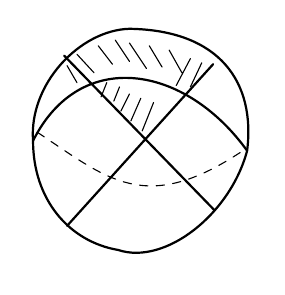
\begin{tikzpicture}[x=0.018cm,y=-0.018cm,line cap=round,line join=round]
\draw[thick] (407,543) .. controls (404,503) and (440,465) .. (475,464) .. controls (539,465) and (564,502) .. (558,550) .. controls (546,595) and (500,631) .. (467,620) .. controls (432,614) and (407,584) .. (407,543) -- cycle;
\draw[thick] (407,543) .. controls (440,477) and (514,489) .. (558,550) (429,483)--(535,592) (431,603)--(534,489);
\draw[dashed] (410,537) .. controls (460,570) and (486,596) .. (555,550);
\draw (431,490)--(438,502) (438,482)--(450,495) (453,476)--(463,489) (465,472)--(475,487) (475,474)--(487,492) (489,476)--(498,491) (503,479)--(512,495) (518,485)--(508,504) (526,488)--(518,505) (459,502)--(455,512) (468,505)--(464,515) (475,510)--(469,522) (483,513)--(476,529) (492,516)--(484,536);
\end{tikzpicture}}

% crop-candidate: scan 96
\figure{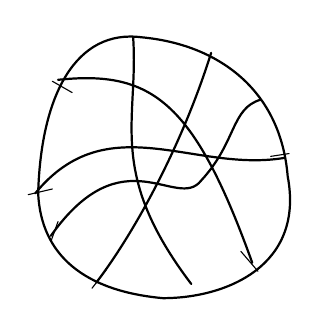
\begin{tikzpicture}[x=0.018cm,y=-0.018cm,line cap=round,line join=round]
\draw[thick] (230,742) .. controls (232,672) and (257,626) .. (303,632) .. controls (357,637) and (401,669) .. (406,730) .. controls (418,793) and (363,816) .. (318,816) .. controls (263,811) and (232,786) .. (230,742) -- cycle;
\draw[thick] (244,662) .. controls (310,655) and (340,677) .. (381,791) (297,632) .. controls (301,691) and (278,727) .. (338,806) (352,643) .. controls (331,710) and (297,771) .. (271,805) (239,772) .. controls (290,700) and (328,755) .. (345,733) .. controls (370,706) and (366,682) .. (387,676) (228,742) .. controls (279,680) and (340,728) .. (404,717);
\draw (240,663)--(254,671) (223,743)--(240,739) (244,762)--(239,776) (268,809)--(278,796) (373,783)--(385,797) (394,716)--(407,714);
\end{tikzpicture}}

% crop-candidate: scan 96
\figure{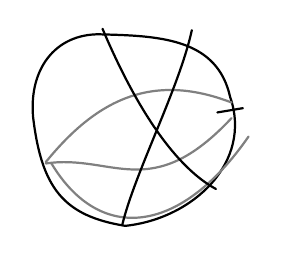
\begin{tikzpicture}[x=0.018cm,y=-0.018cm,line cap=round,line join=round]
\draw[thick] (526,698) .. controls (523,662) and (544,638) .. (576,640) .. controls (618,641) and (656,644) .. (665,684) .. controls (681,730) and (639,770) .. (591,775) .. controls (548,768) and (532,749) .. (526,698) -- cycle;
\draw[gray,thick] (535,730) .. controls (570,687) and (609,666) .. (666,688) (535,731) .. controls (582,724) and (609,760) .. (666,699) (539,731) .. controls (574,789) and (631,780) .. (678,712);
\draw[thick] (575,636) .. controls (603,702) and (631,736) .. (655,749) (638,637) .. controls (629,678) and (598,737) .. (589,774) (656,695)--(674,692);
\end{tikzpicture}}

% crop-candidate: scan 96
\figure{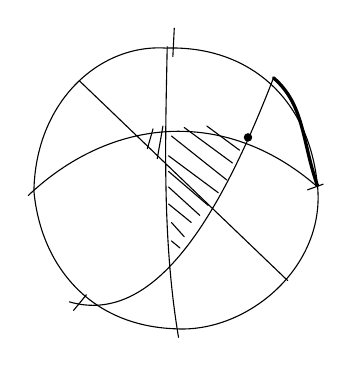
\begin{tikzpicture}[x=0.018cm,y=-0.018cm,line cap=round,line join=round]
\draw[thin] (712,770) .. controls (713,707) and (758,666) .. (805,669) .. controls (862,667) and (906,703) .. (912,766) .. controls (918,823) and (863,870) .. (812,867) .. controls (752,865) and (717,823) .. (712,770) -- cycle;
\draw (744,692)--(891,833) (806,668) .. controls (805,727) and (802,802) .. (814,873) (708,773) .. controls (766,718) and (846,710) .. (911,766) (737,848) .. controls (796,865) and (842,791) .. (881,690);
\draw[very thick] (881,690) .. controls (903,709) and (901,735) .. (912,766);
\fill (863,732) circle[radius=3];\draw (811,655)--(810,675) (740,854)--(749,843) (905,769)--(916,765);
\draw (792,740)--(796,726) (799,747)--(803,724) (809,731)--(848,762) (818,725)--(852,750) (834,724)--(857,741) (807,745)--(842,771) (807,756)--(835,780) (807,767)--(829,787) (807,779)--(823,792) (809,792)--(818,802) (809,805)--(815,810);
\end{tikzpicture}}

% crop-candidate: scan 96
\figure{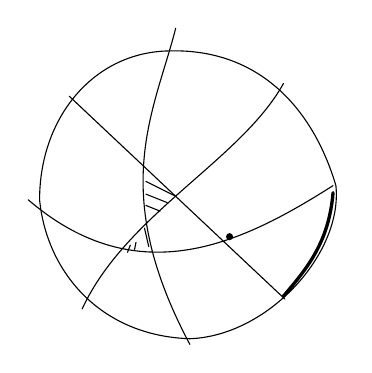
\begin{tikzpicture}[x=0.018cm,y=-0.018cm,line cap=round,line join=round]
\draw[thin] (973,771) .. controls (973,713) and (1011,667) .. (1064,666) .. controls (1128,664) and (1166,707) .. (1182,761) .. controls (1187,809) and (1134,867) .. (1079,869) .. controls (1016,867) and (978,822) .. (973,771) -- cycle;
\draw (994,698)--(1146,841) (1069,650) .. controls (1054,709) and (1021,764) .. (1079,873) (1003,848) .. controls (1034,781) and (1115,743) .. (1145,689) (965,771) .. controls (1043,838) and (1117,801) .. (1180,761);
\draw[very thick] (1180,766) .. controls (1177,801) and (1162,819) .. (1145,839);\fill (1107,797) circle[radius=2.5];\draw (1048,758)--(1068,768) (1048,767)--(1063,773) (1048,775)--(1058,779) (1047,791)--(1050,804) (1041,801)--(1040,806) (1037,803)--(1035,808);
\end{tikzpicture}}

% crop-candidate: scan 96
\figure{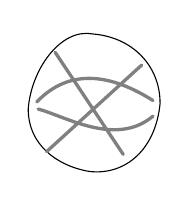
\begin{tikzpicture}[x=0.018cm,y=-0.018cm,line cap=round,line join=round]
\draw (75,845) .. controls (77,817) and (98,788) .. (120,792) .. controls (148,794) and (168,814) .. (168,841) .. controls (165,873) and (144,892) .. (118,889) .. controls (95,885) and (75,870) .. (75,845) -- cycle;
\draw[gray,very thick] (81,840) .. controls (104,816) and (133,820) .. (163,839) (82,845) .. controls (101,850) and (137,872) .. (163,850) (94,805)--(142,877) (88,875)--(155,814);
\end{tikzpicture}}
